\label{sec:fast}

\FAST{} (Facile Aspect-driven Source Transformation) is a novel
language for specifying dataflow designs that are used as a starting
point for the design flow described in Section
\ref{sec:design-flow}. In particular, we use C syntax to capture
dataflow computations but, instead of heavily relying on API libraries
to specify the design (as in MaxCompiler \cite{5719584}), we use
aspect descriptions to specify the transformations required to
optimise the dataflow implementation.

Listing \ref{lst:fast-bscholesr} shows a simple implementation of a
dataflow kernel for finite difference Black-Scholes option pricing
which highlights some of the most important features of \FAST{}:
\begin{itemize}
\item dataflow kernels are declared as regular C functions with inputs
  and outputs clearly defined as arguments in the function signature;
\item \emph{streams} of data are declared and accessed as C99 style pointers;
\item stream ``direction'' (input or output) is inferred by the compiler;
\item type width information is decoupled from the application code
  and can be added automatically via aspect generated pragma
  statements;
\item array indexing is used to access previous, current or past
  stream values;
\item index values are linear combinations of compile-time constants
  or variables;
\item loops with compile-time bounds can be used to parametrise
  dataflow designs;
\item C function calls are mapped to dataflow kernels via pragmas
  which provides the flexibility of selecting a software
  implementation or dataflow configurations based on run-time
  conditions.
\end{itemize}

\begin{lstlisting}[
  style={MaxC},
  label={lst:fast-bscholesr},
  caption={\FAST{} dataflow kernel for European Options pricing}
  ]
  // 1. both input and output streams are declared in kernel header
  // 2. no need for additional type definitions
  void Price_FPGA(float* stockPrices, float *r,
                  float c1, float c2, float c3,
                  int nStocks, int stencilOrder, int timesteps)
  {

    // 3. CURRENT CYCLE value used instead of counter API
    int stockstep  = (CURRENT_CYCLE / n1) \% timesteps;

    #pragma fast DSPBalance:full
    float result = stockPrices[ 0] * c1 + stockPrices[ 1] * c2 + stockPrices[-1] * c3;

    // 4. boolean types used for conditions
    bool up = (stockstep >= stencilOrder) && (stock < stockstep - stencilorder);

    // 5. assigning to output stream automatically outputs value
    r[0] = up ? result : stockPrices;
  }

\end{lstlisting}

\Cref{table:fast-features} summarises the features of \FAST{} and
shows that many are implemented using C syntax. This is
deliberate as it simplifies the programming model and facilitates
direct translation of C applications to dataflow designs.

\begin{table}[!h]
 {\small
  \centering
  \renewcommand{\arraystretch}{1.4}
  \begin{tabularx}{\linewidth}{X|X|p{1.4cm}|X}
    \hline
    \bf{Feature}                        & \bf{Implementation}              & \bf{Method}   & \textbf{Compared to C}      \\
    \hline\hline
    Dataflow Kernels & Function definition & C99 & Cyclic execution \\
    \hline
    I/O                               & Kernel arguments              & Inferred        &  Only params, =  \\
    \hline
    Control                           & Ternary op. (?:), \texttt{if} & C99             &     \\
    \hline
    \multirow{2}{*}{Computation}        & log, exp, sqrt, sin etc.                     & math.h           & Pragmas for range      \\
    &  +, *, /, -     & C99         \\
    \hline
    \multirow{2}{*}{Streams}          & Declared as pointers          & \multirow{2}{*}{C99} &  \multirow{2}{3cm}{Cyclic update; negative offsets } \\
    & Array index access     &                      \\
    \hline
    Optimisation                      & \multirow{2}{*}{C pragmas}    & \multirow{2}{*}{C99} & \multirow{2}{*}{Run-time values}\\
    Hardware \  Mapping               &                               &                      & \\
    \hline
    \multirow{2}{*}{Parameterization} & Constants, variables,         & \multirow{2}{*}{C99}  & \multirow{2}{*}{Compile-time bounds} \\
    & \texttt{for}, \texttt{while}  &                     &  \\
  \end{tabularx}
  \caption{Summary of \FAST{} features.}
  \label{table:fast-features}
}
\end{table}


\FAST{} dataflow designs are compiled by our experimental compiler,
\fastc{} to MaxCompiler designs. \fastc{} extends the
ROSE\cite{Quinlan:2000} compiler framework which is used to produce an
Abstract Syntax Tree(AST) from C sources. The AST is directly
manipulated in a series of compiler passes to generate MaxCompiler
designs for the dataflow kernels. The sequence of passes includes:

\begin{enumerate}
\item \textbf{Extract dataflow kernels} -- separates \FAST{} dataflow
  kernels from the rest of the source C application;
\item \textbf{Constant Extraction} -- extracts design constants from
  source files. These are global constants used to parameterise
  the \FAST{} dataflow designs and can be shared with the CPU
  code;
\item \textbf{Pragma Extraction} -- the pragma extraction pass
  analyses and extracts information from pragmas that specify types of
  streams, ranges of offset streams and other design optimisations;
\item \textbf{Infer input and output streams} -- infers stream direction, as follows:
  \begin{enumerate}
  \item extract kernel parameter set, $P$
  \item extract pointer parameters which form the stream set, $ S \subset P $
  \item perform a written analysis and record the kernel modifies set, $M$
  \item compute the set of output streams, $O = M \cap S$
  \item compute the set of inputs streams, $I = P - O$
  \item detach assignments to output streams from the original AST to
    prevent traversal on future passes and add corresponding output (and
    input) nodes to the dataflow design
  \end{enumerate}
\item \textbf{Inline auxiliary functions} and \textbf{Static Single
    Assignment Renaming} -- inline calls to helper functions
  made from \FAST{} dataflow kernels;
\item \textbf{Type Checking and Inference} -- based on the type of
  input and output streams and values of constants infer and check
  type consistency;
\item \textbf{Dataflow Graph Generation} -- traverse the AST of every
  dataflow kernel to create a corresponding dataflow graph. An example
  generated dataflow graph is shown in \Cref{fig:fast-dfg}. It
  illustrates \texttt{Input}, \texttt{Offset} and \texttt{Arithmetic}
  nodes. The \emph{in} edge of input nodes is connected to a special node
  name \texttt{Source} while the \emph{out} edge of output nodes is
  connected to a special \texttt{Sink} node;
\item \textbf{Remove FAST} -- removes the function nodes corresponding
  to the dataflow kernels from the AST and verifies AST integrity;
\item \textbf{MaxCompiler Design Generation} -- traverse the constructed
  dataflow graph and the original AST to generate corresponding MaxCompiler
  designs for extracted dataflow kernels.
\end{enumerate}

\begin{figure}
  \centering
  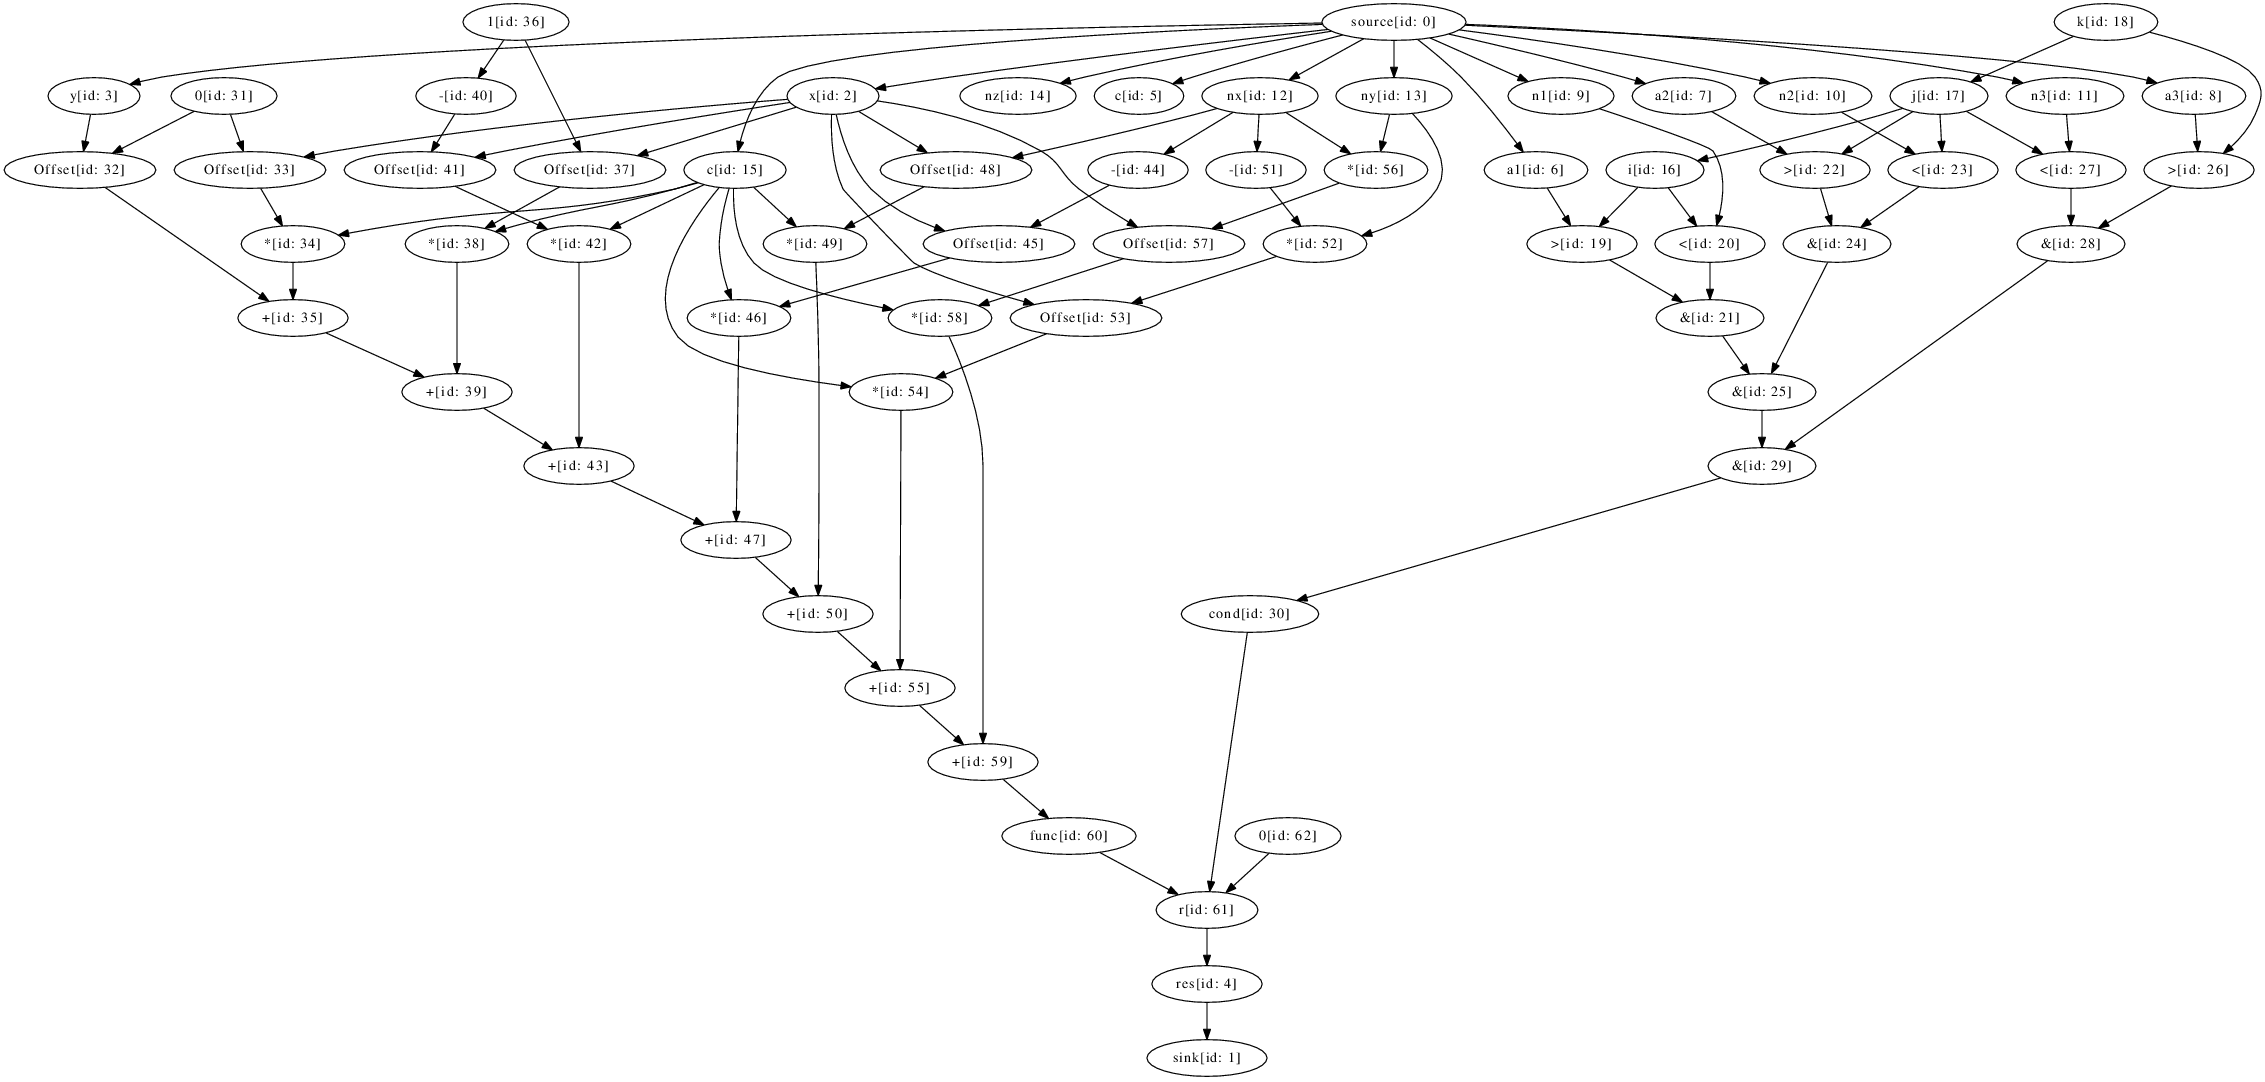
\includegraphics[scale=0.5, clip=true, trim=880 740 650 0]{figs/MaxCtemplateDFG.png}
  \caption{Section of a dataflow graph generated using \fastc{}.}
  \label{fig:fast-dfg}
\end{figure}